\documentclass{article}
\usepackage[UTF8]{ctex}  % 使用中文支持包
\usepackage[a4paper, margin=1in]{geometry}  % 设置纸张大小和边距
\usepackage{anyfontsize}  % 解决字体大小报错问题
\usepackage{fancyhdr}  % 设置页眉、页脚、页码
\usepackage{longtable}  % 支持长表格

\usepackage{amsmath}  % 数学公式支持
\usepackage{cases}  % 支持联立编号
\usepackage{cite}  % 引用支持

\usepackage{graphicx}  % 插入图片支持
\usepackage{float}  % 设置图片浮动位置
\usepackage{subfigure}  % 插入多图时用子图显示

\usepackage{listings}  % 代码块支持
\usepackage{xcolor}  % 设置代码块颜色

\usepackage[hyphens]{url}  % 支持链接换行
\usepackage{hyperref}  % 超链接支持
\usepackage{lastpage}  % 添加lastpage包

\usepackage{gbt7714}  %国标参考文献

\hypersetup{
    hidelinks,
    colorlinks=true,
    allcolors=black,
    pdfstartview=Fit,
    breaklinks=true
}

\title{聚变能源概论-第五讲作业}
\author{\LaTeX\ by\ Jerry\ }
\date{\today}
\pagenumbering{arabic}

\begin{document}
\pagestyle{fancy}

\fancyhead[L]{Jerry}
\fancyhead[C]{聚变能源概论-第五讲作业}
\fancyhead[R]{\today}
\fancyfoot[C]{Page \thepage/\pageref{LastPage}}

\section*{4.6}

\emph{1. 在类似反应堆的条件 $ B_0 = 6 \, T $,密度 $ n = 10^{20} \, m^{-3} $,大半径 $ R = 6 \, m $,小半径 $ a = 2 \, m $, $ \varepsilon = a / R = 1/3 $,拉长比 $ k = 1.7 $,质量数 $ A = 2.5 $,有效电荷 $ Z_{eff} = 1.5 $,归一化安全因子 $ q^* = 1.7 $ 下,分别画出 L 模和 H 模约束下 alpha 粒子加热功率、热传导功率损失、韧致辐射损失功率随温度的变化曲线,并得到稳定和不稳定性的功率平衡点。}

$$\tau_L = 0.037 \frac{\varepsilon^{0.3}}{q_*^{1.7}} \frac{a^{1.17} k^{1.7} B_0^{2.1} A}{n_{20}^{-0.8} T_k} \, [s]$$

$$\tau_H = 0.28 \frac{\varepsilon^{0.74}}{q_*^3} \frac{a^{2.67} k^{3.29} B_0^{3.48} A^{0.61}}{n_{20}^{-0.91} T_k^{2.23}} \, [s]$$

\emph{其中 $ n_{20} $ 单位为 $ 10^{20} \, m^{-3} $,$ T_k $ 单位为 keV。}

如图\ref{fig:1}所示,即为所求。

\begin{figure}[htbp]
    \centering
    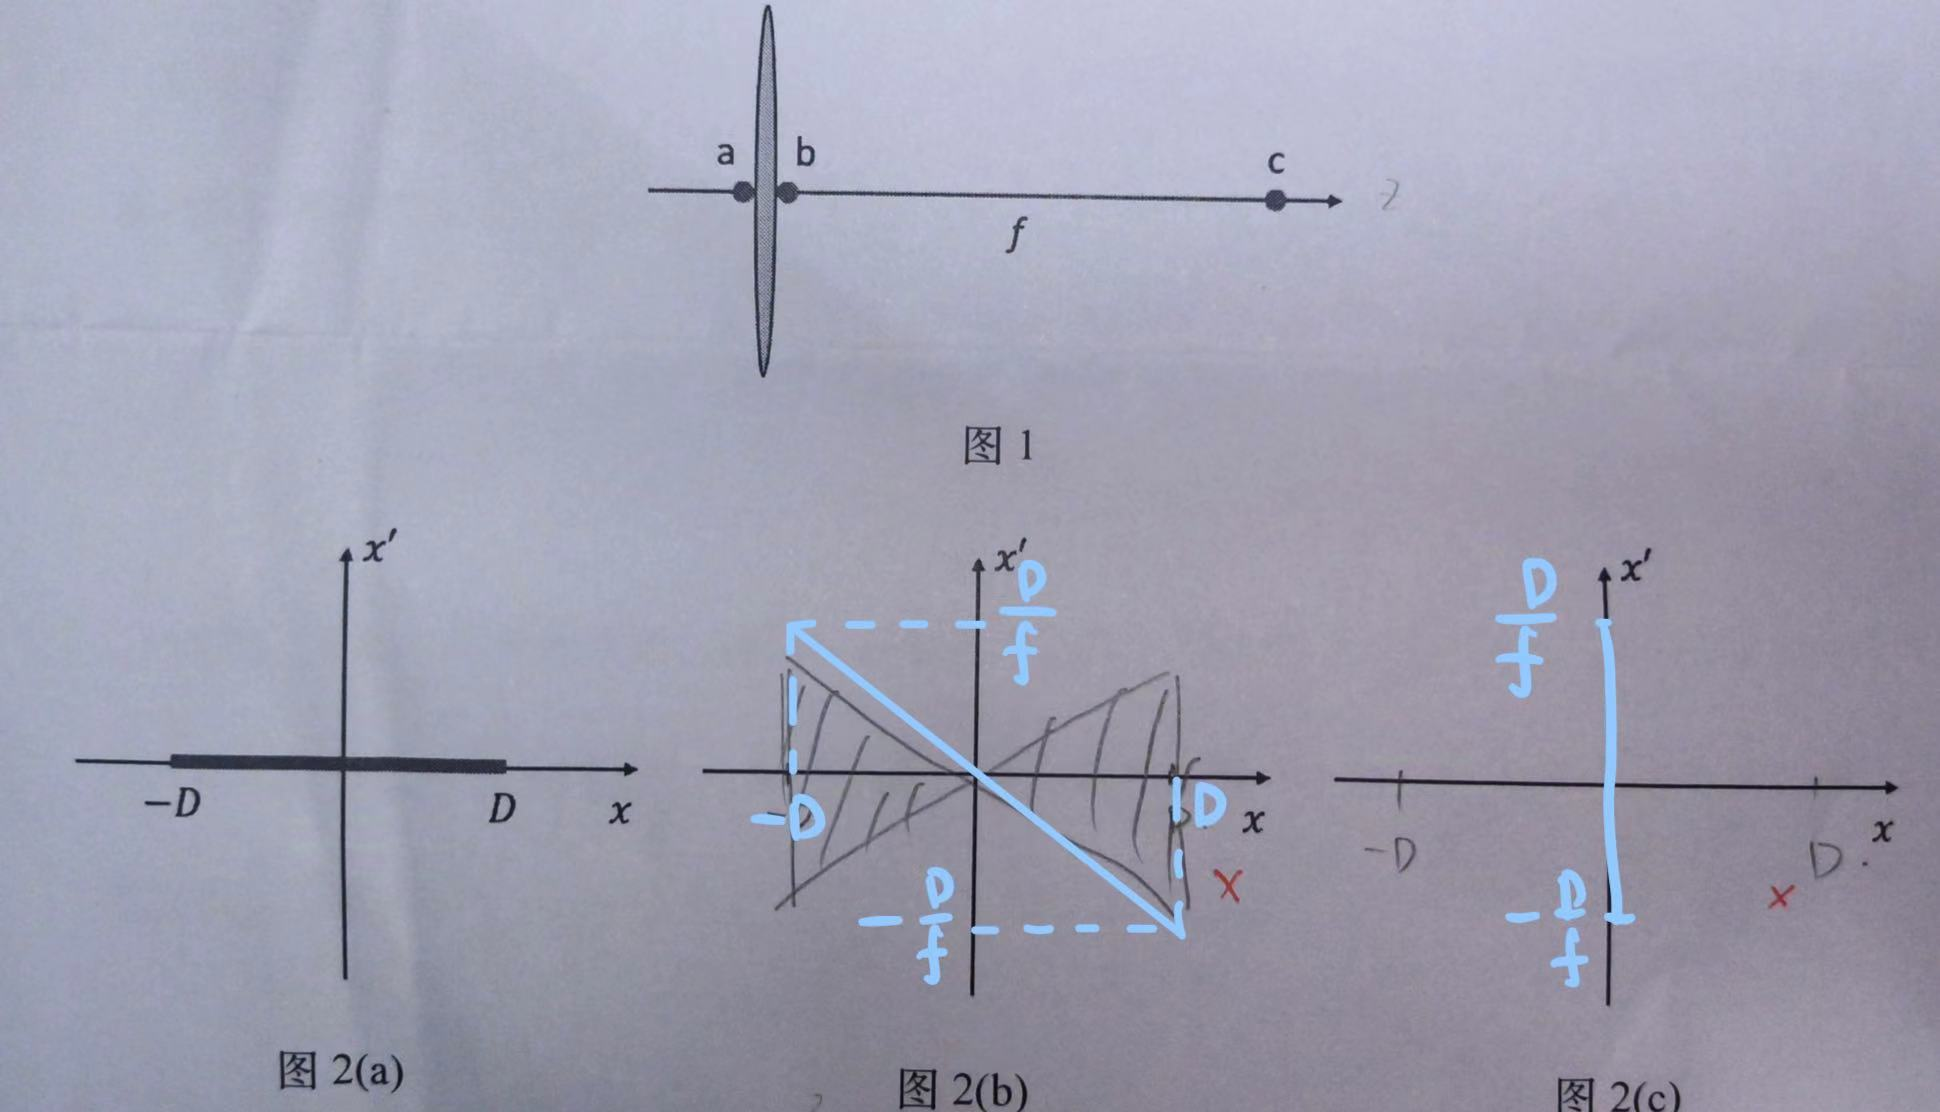
\includegraphics[width=0.8\textwidth]{img/1.pdf}
    \caption{L 模和 H 模约束下 alpha 粒子加热功率、热传导功率损失、韧致辐射损失功率随温度的变化曲线}
    \label{fig:1}
\end{figure}

\section*{4.7}

\emph{2. 在无中子聚变反应中,聚变能量有潜力以更高的效率转化为电能。根据这个特点,仿照课本中对 D-T 反应堆能量流的描述,草拟一个 D-${}^{3}$He 反应堆能量流的框架示意图,并推导在 D-${}^{3}$He 反应堆中工程增益因子和物理增益因子的关系。}

参考教材图4.10, 如图\ref{fig:frame}所示。

\begin{figure}[htbp]
    \centering
    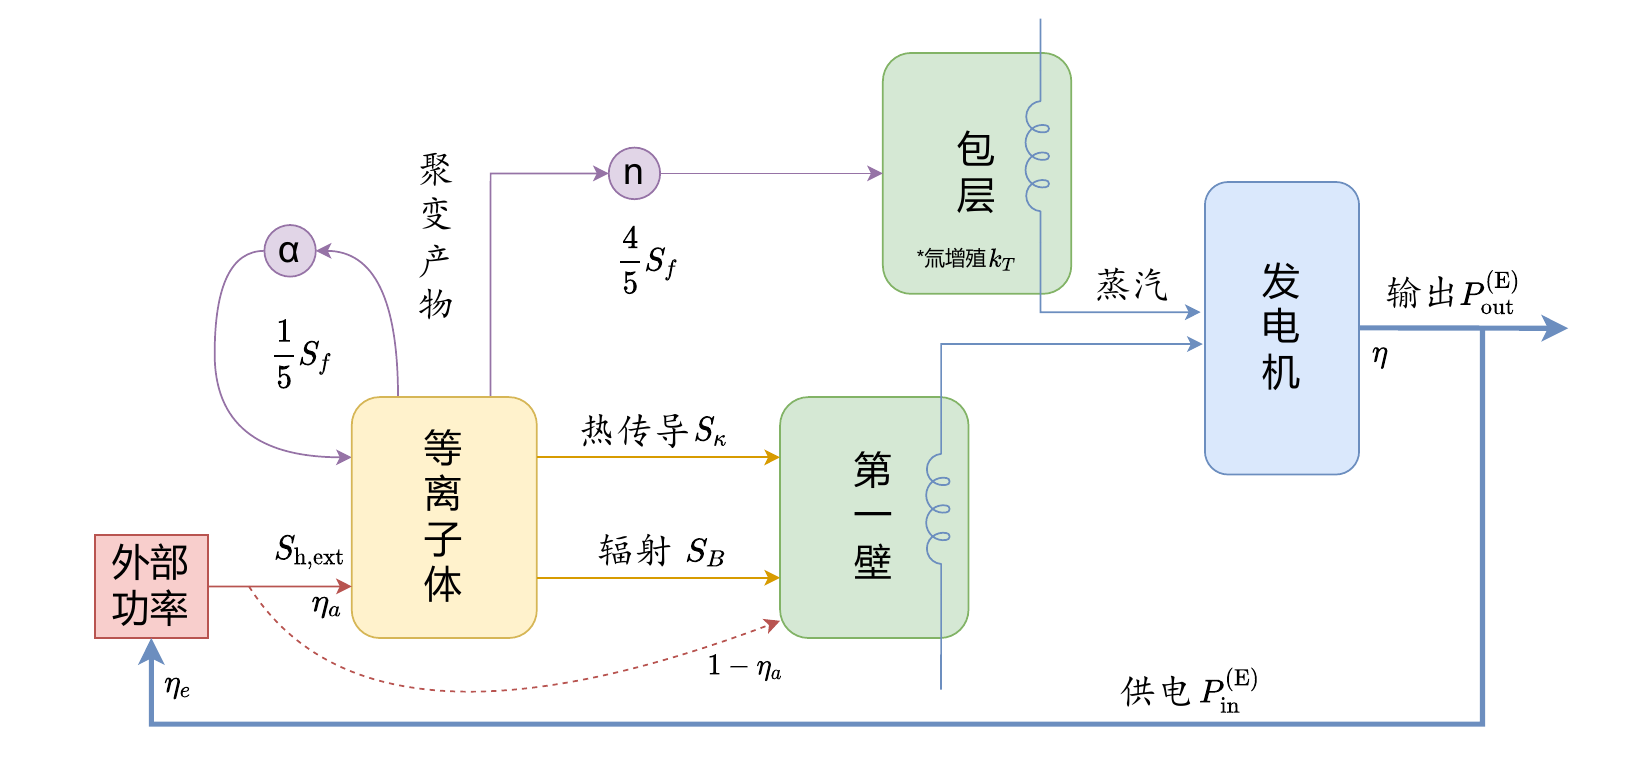
\includegraphics[width=0.8\textwidth]{img/frame.png}
    \caption{D-T 反应堆中能量流的基本框架}
    \label{fig:frame}
\end{figure}

由于反应中无中子流失, 故可以直接忽略中子和包层的能量流。对于反应

$$D + {}^{3}He \rightarrow {}^{4}He + p + 18.3 \, MeV$$

产物获得的能量

$$E(\alpha) = \frac{1}{5} Q = 3.66 \, MeV$$, $$E(p) = \frac{4}{5} Q = 14.64 \, MeV$$

体系功率消耗密度

$$S_{h, ext} = S_\kappa+S_B - S_f$$

取$\eta_a$为等离子体吸收的外部加热功率,$\eta_e$为外部输入电功率的转换效率,则

$$P_{in}^{(H)} = \frac{1}{\eta_a\eta_e}S_{h, ext}V$$

设$\eta_1$为输出热转换电功率,则输出热功率为

$$P_{out}^{(H)} = \eta_1(S_\kappa+S_B+\frac{1-\eta_a}{\eta_a}S_{h, ext})V$$

物理增益因子

$$Q = \frac{P_{out}-P_{in}}{P_{in}} = \frac{S_f}{S_\kappa+S_B - S_f}$$

工程增益因子

$$Q = \frac{P_{out}^{(E)}-P_{in}^{(E)}}{P_{in}^{(E)}} = \frac{(\eta_1\eta_e-1)(S_\kappa+S_B)+(1-\eta_1\eta_e(1-\eta_a))S_f}{S_\kappa+S_B - S_f}$$

\end{document}
